% PAPRIKA pitch deck (7 slides, 5 minutes).
% Build: pdflatex deck.tex (twice). Coordinates are millimetres from the top-left corner of a 160 x 90 mm page.
% Facts: docs/protocol.md, docs/design-rationale.md, docs/limits.md, docs/demo.md, app/README.md.
% Measured numbers: contract/output/cases.md (gas, real UMA contracts on a local chain).
% Amounts and durations are deployment parameters: B, T_photo, T_reveal, f.
% Screenshots: app/output/screens/ (1440 x 900 px, no DPI tag, so 1 px = 1 bp for trim).
\documentclass[aspectratio=169,10pt]{beamer}
\usepackage[T1]{fontenc}
\usepackage{helvet}
\usepackage{tikz}
\usepackage{graphicx}
\usetikzlibrary{calc,arrows.meta}
\definecolor{ink}{HTML}{14123A}
\definecolor{paper}{HTML}{F8F6F1}
\definecolor{lilac}{HTML}{E4DCFB}
\definecolor{lemon}{HTML}{FFF8B8}
\definecolor{mint}{HTML}{C9F2D6}
\definecolor{rose}{HTML}{FFD9D2}
\definecolor{peach}{HTML}{FFE3C7}
\definecolor{sky}{HTML}{DCE6FF}
\definecolor{accent}{HTML}{3B45B5}
\setbeamercolor{background canvas}{bg=paper}
\setbeamercolor{normal text}{fg=ink}
\setbeamertemplate{navigation symbols}{}
\renewcommand{\familydefault}{\sfdefault}
\setbeamertemplate{footline}{}
\hyphenpenalty=10000 \exhyphenpenalty=10000
% --- layout helpers: everything is placed at absolute positions -------------------------------
\newcommand{\at}[2]{($(current page.north west)+(#1mm,-#2mm)$)}
% \card{x}{y}{width}{height}{fill}{content}
\newcommand{\card}[6]{%
  \fill[ink,rounded corners=2.5pt] ($(current page.north west)+(#1mm,-#2mm-0.8mm)$) rectangle ++(#3mm,-#4mm);
  \draw[ink,line width=0.8pt,rounded corners=2.5pt,fill=#5] \at{#1}{#2} rectangle ++(#3mm,-#4mm);
  \node[anchor=north west,inner sep=0pt,text width=#3mm-5mm,align=left,font=\scriptsize] at ($(current page.north west)+(#1mm+2.5mm,-#2mm-2.5mm)$) {#6};}
\newcommand{\head}[2]{%
  \node[anchor=north west,inner sep=0pt,font=\tiny\bfseries] at \at{9}{7} {\MakeUppercase{#1}};
  \node[anchor=north west,inner sep=0pt,font=\LARGE\bfseries] at \at{9}{11} {\MakeUppercase{#2}};
  \node[anchor=south west,inner sep=0pt,font=\tiny\bfseries] at \at{9}{86.5} {PAPRIKA};
  \node[anchor=south east,inner sep=0pt,font=\tiny,text=ink!70] at \at{151}{86.5} {IXH26 $\cdot$ TRACK 1 $\cdot$ \insertframenumber/\inserttotalframenumber};}
\newcommand{\num}[1]{\tikz[baseline=(n.base)]\node(n)[circle,draw=ink,line width=0.7pt,fill=white,inner sep=0.6pt,font=\tiny\bfseries,minimum size=3.4mm]{#1};}
\newcommand{\ct}[1]{{\small\bfseries #1}\\[1mm]}
\tikzset{flow/.style={-{Stealth[length=1.8mm]},line width=0.8pt,draw=ink}}
\newcommand{\headS}[2]{%
  \node[anchor=north west,inner sep=0pt,font=\tiny\bfseries] at \at{9}{7} {\MakeUppercase{#1}};
  \node[anchor=north west,inner sep=0pt,font=\Large\bfseries] at \at{9}{11.5} {\MakeUppercase{#2}};
  \node[anchor=south west,inner sep=0pt,font=\tiny\bfseries] at \at{9}{86.5} {PAPRIKA};
  \node[anchor=south east,inner sep=0pt,font=\tiny,text=ink!70] at \at{151}{86.5} {IXH26 $\cdot$ TRACK 1 $\cdot$ \insertframenumber/\inserttotalframenumber};}
\newcommand{\Tp}{T_{\mathrm{photo}}}
\newcommand{\Tr}{T_{\mathrm{reveal}}}
\tikzset{box/.style={draw=ink,line width=0.8pt,rounded corners=2.5pt,align=left,font=\scriptsize,inner sep=1.6mm,anchor=north west}}
\tikzset{pill/.style={draw=ink,line width=0.7pt,rounded corners=2pt,align=center,font=\tiny,inner sep=1.2mm}}
\begin{document}

% ============================================================ 1 Title
\begin{frame}[plain]
\begin{tikzpicture}[remember picture,overlay]
  \fill[mint] (current page.north west) rectangle \at{70}{90};
  \node[anchor=north west,inner sep=0pt,font=\tiny\bfseries,text width=56mm,align=left] at \at{9}{10} {IXH26 $\cdot$ TRACK 1 $\cdot$ UNIVERSAL PHOTO-ORIGIN VALIDATION PROTOCOL};
  \node[anchor=north west,inner sep=0pt,font=\fontsize{36}{38}\selectfont\bfseries] at \at{8.4}{20} {PAPRIKA};
  \node[anchor=north west,inner sep=0pt,font=\normalsize\bfseries,text width=56mm,align=left] at \at{9}{37} {Photo origin as a claim\\ with money at stake.};
  \node[anchor=north west,inner sep=0pt,font=\small,text width=56mm,align=left] at \at{9}{50} {Signed photos. Money at stake.\\ No manufacturer.};
  \node[anchor=south west,inner sep=0pt,font=\tiny,text=ink!75,text width=60mm,align=left] at \at{9}{84} {Team Sexy Plushies $\cdot$ Francesco Lucibello, Vincenzo Imperati, Lorenzo Camilli};
  \node[anchor=north west,inner sep=0pt,font=\normalsize,text width=74mm,align=left] at \at{78}{14}
    {Apple proves a photo's origin by asking you to trust Apple.\\[2mm]
     Paprika asks you to trust \textbf{no manufacturer}: origin becomes a \textbf{signed claim} with \textbf{money at stake} that \textbf{anyone can challenge}.};
  % running example
  \node[pill,fill=sky]   (al) at \at{88}{52} {\textbf{Alice}\\ signs, locks $B$};
  \node[pill,fill=white] (rc) at \at{108}{52} {public\\ record};
  \node[pill,fill=rose]  (bo) at \at{127}{52} {\textbf{Bob}\\ evidence, $B$};
  \node[pill,fill=lemon] (um) at \at{145}{52} {\textbf{UMA}\\ vote};
  \draw[flow] (al) -- (rc); \draw[flow] (rc) -- (bo); \draw[flow] (bo) -- (um);
  \card{78}{62}{74}{14}{rose}{\textbf{Not claimed:} that a camera took the photo.\\ This is the deliberate price of needing no manufacturer.}
\end{tikzpicture}
\end{frame}

% ============================================================ 2 Reference design
\begin{frame}[plain]
\begin{tikzpicture}[remember picture,overlay]
  \headS{The starting point $\cdot$ Apple Reference Image}{The reference design trusts one company}
  % chain of trust (brief, slides 4-9)
  \node[pill,fill=sky,text width=22mm]   (f1) at \at{21}{31} {3 factory CAs certify sensor and enclave keys};
  \node[pill,fill=lilac,text width=22mm] (f2) at \at{49}{31} {sensor and Secure Enclave sign in hardware};
  \node[pill,fill=lemon,text width=22mm] (f3) at \at{77}{31} {Apple timestamps $[T_0, T_1]$};
  \node[pill,fill=peach,text width=22mm] (f4) at \at{105}{31} {Apple's cloud verifies and signs};
  \node[pill,fill=rose,text width=22mm]  (f5) at \at{133}{31} {Apple keeps the revocation lists};
  \draw[flow] (f1) -- (f2); \draw[flow] (f2) -- (f3); \draw[flow] (f3) -- (f4); \draw[flow] (f4) -- (f5);
  \card{9}{42}{142}{22}{white}{\ct{The brief, slide 10: three weaknesses}
    \textbf{Single point of failure.} ``Apple maintains central revocation lists. A compromised CA invalidates millions of devices.''\\[0.8mm]
    \textbf{Cross-platform lock-in.} ``Non-Apple devices cannot natively verify claims without relying on Apple servers.''\\[0.8mm]
    \textbf{Retroactive censorship.} ``Historic photos become unverifiable if central servers shut down or alter public keys.''}
  \node[anchor=north west,inner sep=0pt,font=\scriptsize,text width=142mm,align=left] at \at{9}{70}
    {Physical origin needs trusted hardware; trusted hardware needs a manufacturer. \textbf{We drop the manufacturer, and we pay for it.}\\[1mm]
     Our test for each weakness: is it \textbf{removed}, or only \textbf{moved}?};
\end{tikzpicture}
\end{frame}

% ============================================================ 3 Protocol
\begin{frame}[plain]
\begin{tikzpicture}[remember picture,overlay]
  \head{The protocol}{Register, attest, challenge, verify}
  \card{9}{24}{33.5}{22}{sky}{\num{1} \textbf{REGISTER} (free)\\[0.8mm] Alice's key signs Alice's address: proof of possession.}
  \card{45.2}{24}{33.5}{22}{lilac}{\num{2} \textbf{ATTEST}\\[0.8mm] The key signs $H(\mathit{photo})$ and $\mathrm{blockhash}(a)$. Alice locks $B$.}
  \card{81.4}{24}{33.5}{22}{rose}{\num{3} \textbf{CHALLENGE}\\[0.8mm] Until $r + \Tp$: Bob commits, then reveals, with bond $B$. UMA votes.}
  \card{117.6}{24}{33.4}{22}{mint}{\num{4} \textbf{OUTCOME}\\[0.8mm] The loser loses $B$; the winner gets $B - fB$ of it. No challenge: Alice gets $B$ back.}
  % time axis
  \draw[ink,line width=0.9pt,-{Stealth[length=1.8mm]}] \at{12}{58} -- \at{150}{58};
  \foreach \x/\l in {20/{block $a$\\anchor}, 48/{block $r$\\record, $B$ locked}, 96/{$r + \Tp$\\last commitment}, 128/{$+\,\Tr$\\refund possible}}{
    \draw[ink,line width=0.9pt] \at{\x}{56.5} -- \at{\x}{59.5};
    \node[anchor=south,font=\tiny,align=center,inner sep=0.5pt] at \at{\x}{56.3} {\l};}
  \fill[lilac!80] \at{20}{57.6} rectangle \at{48}{58.4};
  \node[pill,fill=rose,anchor=north] (cm) at \at{66}{62} {Bob: commit $\to$ reveal $\to$ UMA vote};
  \node[pill,fill=white,anchor=north west] (np) at \at{98}{61.5} {not proven: period extended};
  \node[pill,fill=white,anchor=north west] (fk) at \at{98}{66.5} {fake proven: record Fake, key flagged};
  \draw[flow] (cm.east) -- (np.west); \draw[flow] (cm.east) -- (fk.west);
  \card{9}{72}{142}{8}{white}{\textbf{Verify: anyone} hashes the file and reads the contract. No account, no transaction, no server.
    {\color{ink!70}One contract; no owner, no admin key; Paprika takes no fee. Parameters fixed at deployment.}}
\end{tikzpicture}
\end{frame}

% ============================================================ 4 Cryptography
\begin{frame}[plain]
\begin{tikzpicture}[remember picture,overlay]
  \head{The cryptography}{What it proves, and what it does not}
  \node[anchor=north west,inner sep=0pt,font=\scriptsize,text width=142mm,align=left] at \at{9}{24}
    {$\sigma = \mathrm{Sig}_K(\texttt{"PAPRIKA/CAPTURE"} \| \mathit{chainId} \| \mathit{contract} \| \mathit{keyId} \| H \| \mathrm{blockhash}(a))$\quad ECDSA P-256, low-$s$, checked on chain by the precompile (EIP-7951).};
  \card{9}{31}{68}{27}{mint}{\ct{A record proves}
    $\bullet$ key $K$ signed this exact file $H$\\
    $\bullet$ after block $a$: a block hash is unpredictable\\
    $\bullet$ the file existed by block $r$\\
    $\bullet$ the signature is bound to this chain and contract\\
    $\bullet$ $B$ is at stake}
  \card{81}{31}{70}{27}{rose}{\ct{A record does not prove}
    $\bullet$ that a camera took the photo\\
    $\bullet$ that the key lives in protected hardware (the demo key is a software key)\\
    $\bullet$ when the scene was captured: an old file can be signed today\\
    $\bullet$ who Alice is}
  % evidence figure
  \draw[ink,line width=0.9pt,-{Stealth[length=1.6mm]}] \at{12}{74} -- \at{80}{74};
  \fill[lilac] \at{46}{73} rectangle \at{62}{75};
  \node[font=\tiny,anchor=north] at \at{46}{75.5} {block $a$}; \node[font=\tiny,anchor=north] at \at{62}{75.5} {block $r$};
  \node[font=\tiny,anchor=south] at \at{54}{75.2} {};
  \node[font=\tiny,anchor=north west,inner sep=0pt] at \at{48}{69.5} {signing window};
  \draw[flow,draw=accent] \at{24}{68.8} -- \at{24}{73.3};
  \node[font=\tiny,anchor=north,align=center,text=accent,inner sep=0pt] at \at{24}{62.5} {Bob's evidence: the same image\\ was public \textbf{before} $a$};
  \node[anchor=north west,inner sep=0pt,font=\scriptsize,text width=66mm,align=left] at \at{85}{61}
    {\textbf{Bob's commitment}\\ \mbox{$c = \mathrm{keccak}(\mathit{Bob} \| H \| \mathit{keyId} \| H(\mathit{evidence}) \| \mathit{salt})$}\\ hides the target and names Bob. A copy cannot be revealed. The reveal comes at least one block later.\\[1mm]
     \textbf{Several keys may attest one file.} The verifier lists them and judges each key.};
\end{tikzpicture}
\end{frame}

% ============================================================ 5 Who pays
\begin{frame}[plain]
\begin{tikzpicture}[remember picture,overlay]
  \head{The mechanism}{Who pays when someone is wrong}
  \node[anchor=north west,inner sep=0pt,font=\scriptsize,text width=142mm,align=left] at \at{9}{23}
    {Paprika \textbf{asserts} Bob's accusation at UMA's Optimistic Oracle V3 with Bob's bond, and \textbf{disputes} it in the same transaction with Alice's deposit. Every accusation goes to UMA's vote; none wins by silence.};
  \card{9}{31}{80}{36}{white}{\ct{UMA's question and the payoffs}
    ``Is this photo not a genuine capture by key $K$?'' Voters say yes only if the claim is \textbf{true and publicly verifiable} (UMIP-170). \textbf{The burden of proof is on Bob.}\\[1.2mm]
    \renewcommand{\arraystretch}{1.25}
    \begin{tabular}{@{}p{16mm}p{14mm}p{34mm}@{}}
      & \textbf{Bob} & \textbf{Alice}\\
      \textbf{Fake proven} & $+B - fB$ & $-B$; record Fake; key flagged\\
      \textbf{Not proven} & $-B$ & $+B - fB$; period extended\\
    \end{tabular}\\[1mm]
    {\color{ink!70}$f$: UMA's share of the loser's stake, set by UMA. Paprika takes nothing.}}
  \card{93}{31}{58}{36}{peach}{\ct{Deterrence, honestly}
    \textbf{Self-accusation.} A forger who expects to be caught accuses its own fake from a second account, with the real evidence. It loses $fB$, not $B$.\\[1mm]
    \textbf{Revealing ahead of Bob.} A forger holding an older commitment can reveal before Bob. Bob gets his bond back, no reward; the fake is still proven.\\[1mm]
    Expected punishment: between $p\,fB$ and $p\,B$.}
  \node[anchor=north west,inner sep=0pt,font=\scriptsize,text width=142mm,align=left] at \at{9}{70.5}
    {The reward is the forger's own deposit: no shared pool to drain. A fake worth more than the punishment is not deterred, so $B$ must be sized to what a fake is worth.};
  \node[anchor=north west,inner sep=0pt,font=\tiny,text width=142mm,align=left] at \at{9}{79}
    {\textbf{Related work.} Deposits forfeited by \emph{cryptographic} proof: Kiayias and Tang (CCS 2013, 2015); Ruffing, Kate and Schr\"oder (CCS 2015). ``Fake'' has no cryptographic proof, so here a vote decides.};
\end{tikzpicture}
\end{frame}

% ============================================================ 6 Demo
\begin{frame}[plain]
\begin{tikzpicture}[remember picture,overlay]
  \head{Live demo}{Alice attests, Bob accuses, UMA decides}
  % app/output/screens/04-verifier-attested.png and 14-verifier-proven-fake.png (crops of the verifier panel)
  \node[anchor=north west,inner sep=0pt] at \at{9}{24} {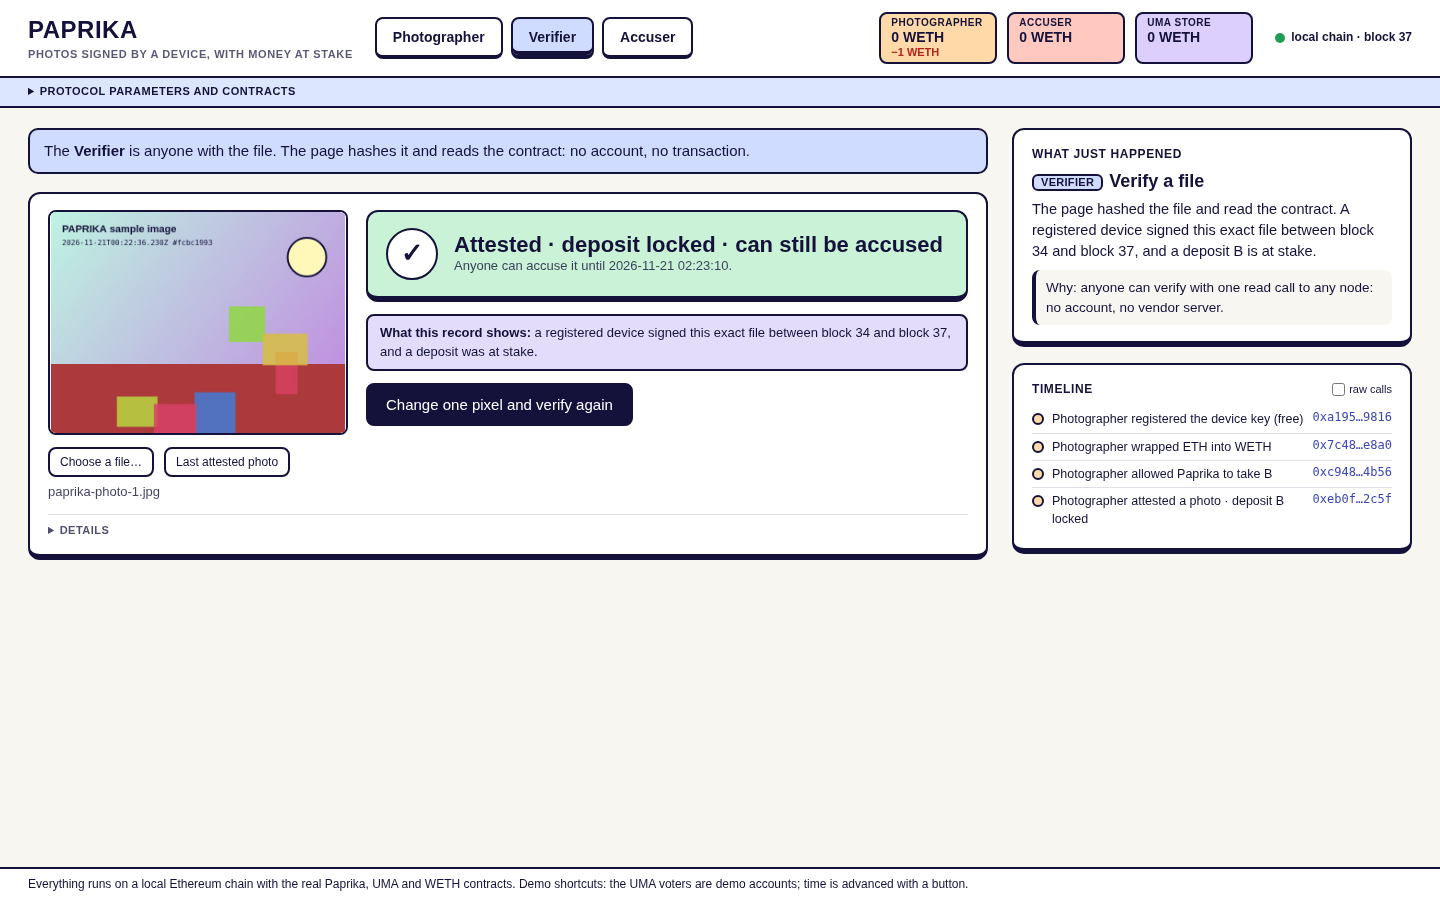
\includegraphics[width=88mm,trim=48 455 472 210,clip]{../app/output/screens/04-verifier-attested.png}};
  \node[anchor=north west,inner sep=0pt] at \at{9}{50} {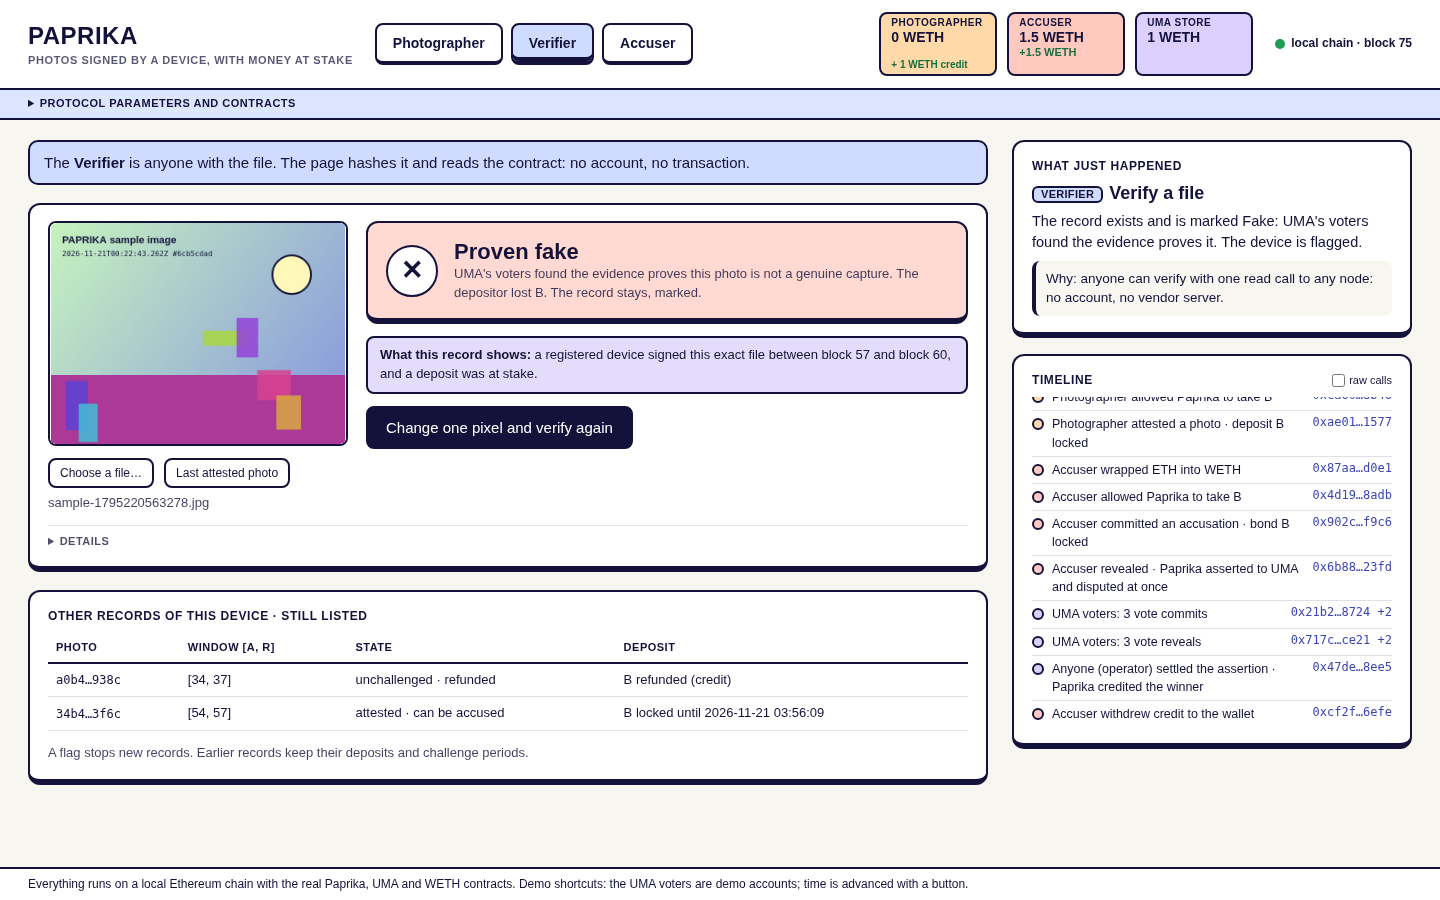
\includegraphics[width=88mm,trim=48 444 472 222,clip]{../app/output/screens/14-verifier-proven-fake.png}};
  \draw[ink,line width=0.6pt] \at{9}{24} rectangle \at{97}{46.5};
  \draw[ink,line width=0.6pt] \at{9}{50} rectangle \at{97}{73};
  \node[anchor=north west,font=\tiny\bfseries,inner sep=0pt] at \at{9}{47.3} {Before: signed, staked, open to challenge};
  \node[anchor=north west,font=\tiny\bfseries,inner sep=0pt] at \at{9}{73.8} {After UMA's vote: proven fake, record kept};
  \card{101}{24}{50}{52}{white}{\ct{The click path}
    \num{1}\; Register a key (free)\\[0.9mm]
    \num{2}\; Attest; lock $B$\\[0.9mm]
    \num{3}\; Verify: signed, staked, open\\[0.9mm]
    \num{4}\; Change one pixel: no record\\[0.9mm]
    \num{5}\; Bob commits, then reveals\\[0.9mm]
    \num{6}\; UMA votes: fake proven\\[0.9mm]
    \num{7}\; Verify again: proven fake, record kept}
  \node[anchor=north west,inner sep=0pt,font=\tiny,text=ink!75,text width=142mm,align=left] at \at{9}{78.3}
    {Local Ethereum chain: Paprika, WETH, and UMA's Optimistic Oracle V3 and voting contracts. Three demo voter accounts; chain clock advanced by a button.
     Demo values: $B$ = 1 WETH, $\Tp$ = 1\,h, $\Tr$ = 15\,min.}; % app/README.md, parameter defaults (BOND 1, PHOTO_WINDOW 3600, REVEAL_WINDOW 900)
\end{tikzpicture}
\end{frame}

% ============================================================ 7 Removed, moved, not claimed
\begin{frame}[plain]
\begin{tikzpicture}[remember picture,overlay]
  \head{Back to the test}{Removed, moved, and not claimed}
  \card{9}{23}{80}{36}{white}{\ct{Removed or moved}
    \textbf{Single point of failure.} No CA, no central revocation list, no owner. \emph{Moved} to UMA's vote, which can err or be bought; one vote touches one record and one key.\\[1mm]
    \textbf{Lock-in.} Any P-256 key registers; any node verifies. \emph{Remains:} one public chain.\\[1mm]
    \textbf{Retroactive censorship.} No record or key is ever deleted; flags carry their block.\\[1mm]
    {\color{ink!70}Trust is moved, not eliminated.}}
  \card{93}{23}{58}{36}{rose}{\ct{Not claimed}
    $\bullet$ physical origin\\
    $\bullet$ fakes that leave no public evidence\\
    $\bullet$ fakes worth more than the deposit\\
    $\bullet$ a flagged party returns with a free new key\\
    $\bullet$ exact file only: a recompressed copy has no record\\
    $\bullet$ records of one key are linkable\\
    $\bullet$ each vote takes 48--72\,h on a real network % docs/limits.md, "What UMA can and cannot do" (UMA docs: "within 48-72 hours")
    }
  \node[anchor=north west,inner sep=0pt,font=\scriptsize,text width=142mm,align=left] at \at{9}{62.5}
    {\textbf{Good for:} low-value fakes that leave public traces: sale listings, recycled photos. \textbf{Not enough alone for} news or legal evidence.\\
     \textbf{Next:} unlinkable records (a zero-knowledge proof of membership in the set of unflagged keys); batching many photos under one deposit.};
  \card{9}{74}{142}{8}{white}{\textbf{AI disclosure.} Design, code, documentation and slides made with Claude Code (Anthropic) under the team's direction. Log: \texttt{AI\_DISCLOSURE.md}.}
\end{tikzpicture}
\end{frame}
\end{document}
